\documentclass{pracamgr}  
\usepackage{lmodern} 
\usepackage[polish]{babel} 
\selectlanguage{polish} 
\usepackage{fontspec}
\usepackage{minted}
\usepackage{listings}
% package for hyperinks
\usepackage{hyperref}
\hypersetup{
    colorlinks,
    citecolor=black,
    filecolor=black,
    linkcolor=black,
    urlcolor=black
}
   
\definecolor{grey}{gray}{0.9}
\definecolor{bg}{HTML}{FAFAFA}
\definecolor{darkgray}{HTML}{D5D5D5}

\makeatletter
\renewenvironment{minted@colorbg}[1]{
\setlength{\fboxsep}{\z@}
\def\minted@bgcol{#1}
\noindent
\begin{lrbox}{\minted@bgbox}
\begin{minipage}{\linewidth}}
{\end{minipage}
\end{lrbox}%
\colorbox{\minted@bgcol}{\usebox{\minted@bgbox}}}
\makeatother

% Dane magistranta:

\author{Konrad Lisiecki}
\nralbumu{291649}
\title{Mechanizmy funkcyjne w języku C++}
\tytulang{Functional programming in C++}
\kierunek{Informatyka}

\opiekun{dra Marcina Benke\\
  Instytut Informatyki\\
}
\date{Warszawa 2015}
\dziedzina{ 
  11.3 Informatyka\\ 
}
\klasyfikacja{D. Software\\
  D.1 Programming techniques\\
  D.1.1 Applicative (Functional) Programming}
\keywords{C++, functional programming, C++11, funkcja lambda}
\newtheorem{defi}{Definicja}[section]

\begin{document}

\maketitle

\begin{abstract}
Celem pracy magisterskiej jest kompleksowe przedstawienie mechanizmów programowania 
funkcyjnego, które zostały wprowadzone do najnowszych standardów języka C++. Autor pracy skupi się
na sposobie realizacji wprowadzonych mechanizmów oraz zbadaniu siły ich wyrazu. 
W ramach pracy zostanie również dokonane ich porównanie z rozwiązaniami istniejącymi w innych 
językach programowania, jak python i haskell.
\end{abstract}


\tableofcontents


\chapter*{Wprowadzenie}
\addcontentsline{toc}{chapter}{Wprowadzenie}


Język C++ jest jednym z najbardziej popularnych języków programowania.
Powszechnie uważa się, że zastosowano w nim trzy paradygmaty programowania: programowanie imperatywne, obiektowe i generyczne.
Jednak w standardzie C++11 wprowadzono wiele mechanizmów funkcyjnych, znanych z innych języków programowania.

Właśnie o wprowadzonych mechanizmach funkcyjnych do języka C++ traktuje poniższa praca.

Składa się ona z czterech rozdziałów i dodatków.
W rozdziale~\ref{r:Zmiany} opisano najważniejsze zmiany jakie wprowadzono do nowego standardu języka C++.
Rozdział~\ref{r:SposobRealizacji} przedstawia sposób wprowadzenia zmian do języka oraz siłę ich wyrazu. 
Wprowadzone zmiany zostaną dokładnie opisane pod względem generyczności i szybkości rozwiązania.


Kolejna część pracy (rozdział \ref{r:Porownanie}) porównuje efektywność i szybkość działania programu.
Zostanie porównana szybkość działania konstrukcji funkcyjnych z tymi spotykanymi w języku Haskell i Python.

Rozdział \ref{r:Biblioteka} zawiera z kolei krótki opis biblioteki zaimplementowanej przy użyciu technik 
metaprogramowania. Jest to biblioteka dostarczająca gotowych funkcji do operowania na listach. Jest ona 
zaimplementowana w duchu biblioteki LINQ, obecnej w języku $C\#$. 


W ostatnim rozdziale jest zawarte podsumowanie wprowadzonych zmian. 
W dodatkach z kolei, umieszczono wybrane fragmenty kodu zaimplementowanej biblioteki z rozdziału \ref{r:Biblioteka}.






\chapter{Opis wprowadzonych zmian do języka C++}\label{r:Zmiany}

W niniejszym rozdziale zostaną przedstawione najważniejsze zmiany jakie wprowadzono do języka C++ w nowych standardach. 
Szczególna uwaga zostanie jednak zwrócona na mechanizmy, które są charakterystyczne dla programowania w stylu funkcyjnym.
Należy tutaj wymienić przede wszystkim funkcje lambda oraz automatyczne określanie typu przy pomocy słowa kluczowego \textit{auto}.





\section{Funkcje lambda}

Funkcje lambda, chociaż nie zwiększają siły wyrazu języka C++, mają olbrzymi wpływ na jakość pisanego 
oprogramowania.

Obecnie nie ma potrzeby definiowania nowej funkcji z nazwy, można po prostu użyć funkcji lambda.
Efektem jest znaczące uproszczenie kodu, co czyni go bardziej czytelnym i napisanym w bardziej funkcyjnym stylu.
 
Dla przykładu porównajmy więc przykładową funkcję z biblioteki standardowej z użyciem funkcji lambda i bez niej.
I tak, poniższy listing przedstawia funkcję \textit{find\_if} z użyciem funkcji lambda: 

\begin{listing}[ht]
\inputminted[mathescape, linenos, numbersep=5pt, bgcolor=bg, rulecolor=\color{darkgray}, frame=lines, framesep=2mm]{cpp}
{listings/lambda0.cpp}
\caption{Przykład użycia funkcji anonimowej}
\label{lst:HigherOrderPython}
\end{listing}

\noindent
Składnia funkcji lambda składa się z 4 podstawowych elementów
\begin{enumerate}
\item definicji domknięcia (ang. closure),
\item listy z parametrami
\item typu zwracanego (opcjonalnie)
\item bloku z kodem
\end{enumerate}

\noindent
które mają następującą składnię:

\begin{listing}[H]
\inputminted[mathescape, linenos, numbersep=5pt, bgcolor=bg, rulecolor=\color{darkgray}, frame=lines, framesep=2mm]{cpp}
{listings/lambdaSyntax.cpp}
\caption{Przykład użycia funkcji anonimowej}
\label{lst:lambdaSyntax}
\end{listing}

W konstrukcji tej najważniejszym elementem jest definicja domknięcia. To w niej możemy 
specyfikować do jakich zmiennych i w jakim trybie mamy dostęp wewnątrz funkcji.
Generalnie są do dyspozycji następujące typy dostępu do zmiennych w funkcji:
\begin{enumerate}
\item  - \textbf{[a,&b]}, a dostępne przez wartość, b przez referencję.
\item  - \textbf{[this]}, wskaźnik do this jest dostępny do przez wartość
\item  - \textbf{[&]}, przekazuje wszystkich zmienne przez referencję
\item  - \textbf{[=]}, przekazuje wszystkich zmienne przez wartość
\item  - \textbf{[]}, nie są przekazane żadne zmienne do funkcji
\end{enumerate}

Poniższy listing nr \ref{lst:lambdaUsage} wskazuje na kilka poprawnych i niepoprawnych sposobów użycia
funkcji anonimowych

\begin{listing}[ht]
\inputminted[mathescape, linenos, numbersep=5pt, bgcolor=bg, rulecolor=\color{darkgray}, frame=lines, framesep=2mm]{cpp}{lambda1.cpp}
\caption{Przykład poprawnego i niepoprawnego użycia capture-list w wyrażeniach lambda}
\label{lst:lambdaUsage}
\end{listing}



\section{Automatyczne określanie typu}
 
Kolejnym cechą wprowadzoną do C++, a która jest powszechnie używana w językach funkcyjnych, jest automatyczne
określanie typu (ang. \textit{type inference}). W C++ do osiągnięcia tego celu wprowadzono słowo kluczowe \textit{auto}.
Podczas deklaracji zmiennej z automatycznym określeniem typu musimy od razu zainicjalizować, tak aby, kompilator 
potrefił określić typ tej zmiennej. Obrazuje to poniższy listing nr \ref{lst:auto}: 

\begin{listing}[H]
\inputminted[mathescape, linenos, numbersep=5pt, bgcolor=bg, rulecolor=\color{darkgray}, frame=lines, framesep=2mm]{cpp}{listings/auto.cpp}
\caption{Przykład poprawnego i niepoprawnego użycia capture-list w wyrażeniach lambda}
\label{lst:auto}
\end{listing}

Pomimo olbrzymiej prostoty, która wiąże się z użyciem deklaracji typu \textit{auto}, 
należy pamiętać, że w pewnych sytuacjach
wyznaczony typ może być nieprawidłowy. Taka sytuacja występuje podczas użycia w kodzie programu wzorca 
projektowego pełnomocnik (ang. \textit{proxy}).
Rozwiązaniem tego problemu jest użycie wprost typowanego inicjalizatora (ang. \textit{explicitly typed initializer idiom}).

Jednak weźmy pod uwagę następującą funkcję

\begin{listing}[H]
\inputminted[mathescape,  numbersep=5pt, bgcolor=bg, rulecolor=\color{darkgray}, frame=lines, framesep=2mm]{cpp}{listings/auto/auto1.cpp}  
\end{listing}

i przypuśćmy, że chcielibyśmy osłabić zwracany typ z \textit{double} do \textit{float}.

Powstaje więc pytanie, dlaczego nie moglibyśmy po prostu dokonać niejawnej konwersji typu:

\begin{listing}[H]
\inputminted[numbersep=5pt, bgcolor=bg, rulecolor=\color{darkgray}, frame=lines, framesep=2mm]{cpp}{listings/auto/auto2.cpp}  
\end{listing}

zamiast użycia wprost typowanego inicjalizatora:


\begin{listing}[H]
\inputminted[numbersep=5pt, bgcolor=bg, rulecolor=\color{darkgray}, frame=lines, framesep=2mm]{cpp}{listings/auto/auto3.cpp}  
\end{listing}

Argument za tym drugim rozwiązaniem jest związany z czytelnością kodu. Wykorzystując wprost typowany incjalizator 
\textit{explicite} mówimy, że zmieniamy typ wyrażenia. Dlatego tak napisany kod jest bardziej przejrzysty: mówimy 
wprost, że chcemy dokonać konwersji typu.









\section{Funkcje obywatelami pierwszej kategorii}

Wraz z pojawieniem się funkcji anonimowych funkcje stały się obywatelami pierwszej kategorii w języku C++.

\begin{listing}[ht]
\inputminted[mathescape, linenos, numbersep=5pt, bgcolor=bg, rulecolor=\color{darkgray}, frame=lines, framesep=2mm]{cpp}{firstCategory.cpp}
\caption{Przykład poprawnego i niepoprawnego użycia capture-list w wyrażeniach lambda}
\label{listing:3}
\end{listing}






\section{Funkcje wyższego rzędu}


Funkcje wyższego rzędu, czyli funkcje, które przyjmują jako argument lub zwracają funkcje, są 
podstawowym narzędziem w każdym programie funkcyjnym. 
Także w C++ mamy do dyspozycji wiele funkcji wyższego rzędu w STL-u.


\subsection{Funkcje wbudowane}
Jednakże, prowadzenie do standardu C++11 funkcji anonimowych znaczenie ułatwiło korzystanie z wielu wbudowanych, STL-owych funkcji, 
takich jak:
\begin{enumerate}
\item \textit{trasform}
\item \textit{remove\_if}
\item \textit{accumulate}
\end{enumerate}

\noindent
I tak, poniższy listing nr \ref{lst:accumulate} przedstawia przykładową implementację funkcji \textit{accumulate}:

\begin{listing}[H]
\inputminted[mathescape, linenos, numbersep=5pt, bgcolor=bg, rulecolor=\color{darkgray}, frame=lines, framesep=2mm]{cpp}{accumulate.cpp}
\caption{Definicja funkcji accumulate}
\label{lst:accumulate}
\end{listing}


Jak widzimy w definicji funkcji jako ostatni argument mamy pewną binarną funkcję, którą możemy
zdefiniować przy pomocy funkcji anonimowej.

\subsection{Programowanie aspektowe}

Programowanie aspektowe, jako kolejny paradygmat programowania, znacząco ułatwia podzielenie programu na części będącą ze sobą nawzajem niezależne. 
Gdy 
Rysunek \ref{fig:aspektProgramming} przedstawia ideę stojącą za programowaniem aspektowym i sposób w jaki następuje połączenie niezależnych ze sobą części. 

Dlaczego w rozdziale poświęconym funkcjom wyższego rzędu piszemy o programowaniu aspektowym? Z tego względu, że znacznie one pomagają tworzenie programów 
zgodnym z duchem programowania aspektowego. 

Weźmy np. funkcjonalność logowania, które jest obecne właściwie w każdym większym projekcie programistycznym.


\begin{figure}
  \centering
  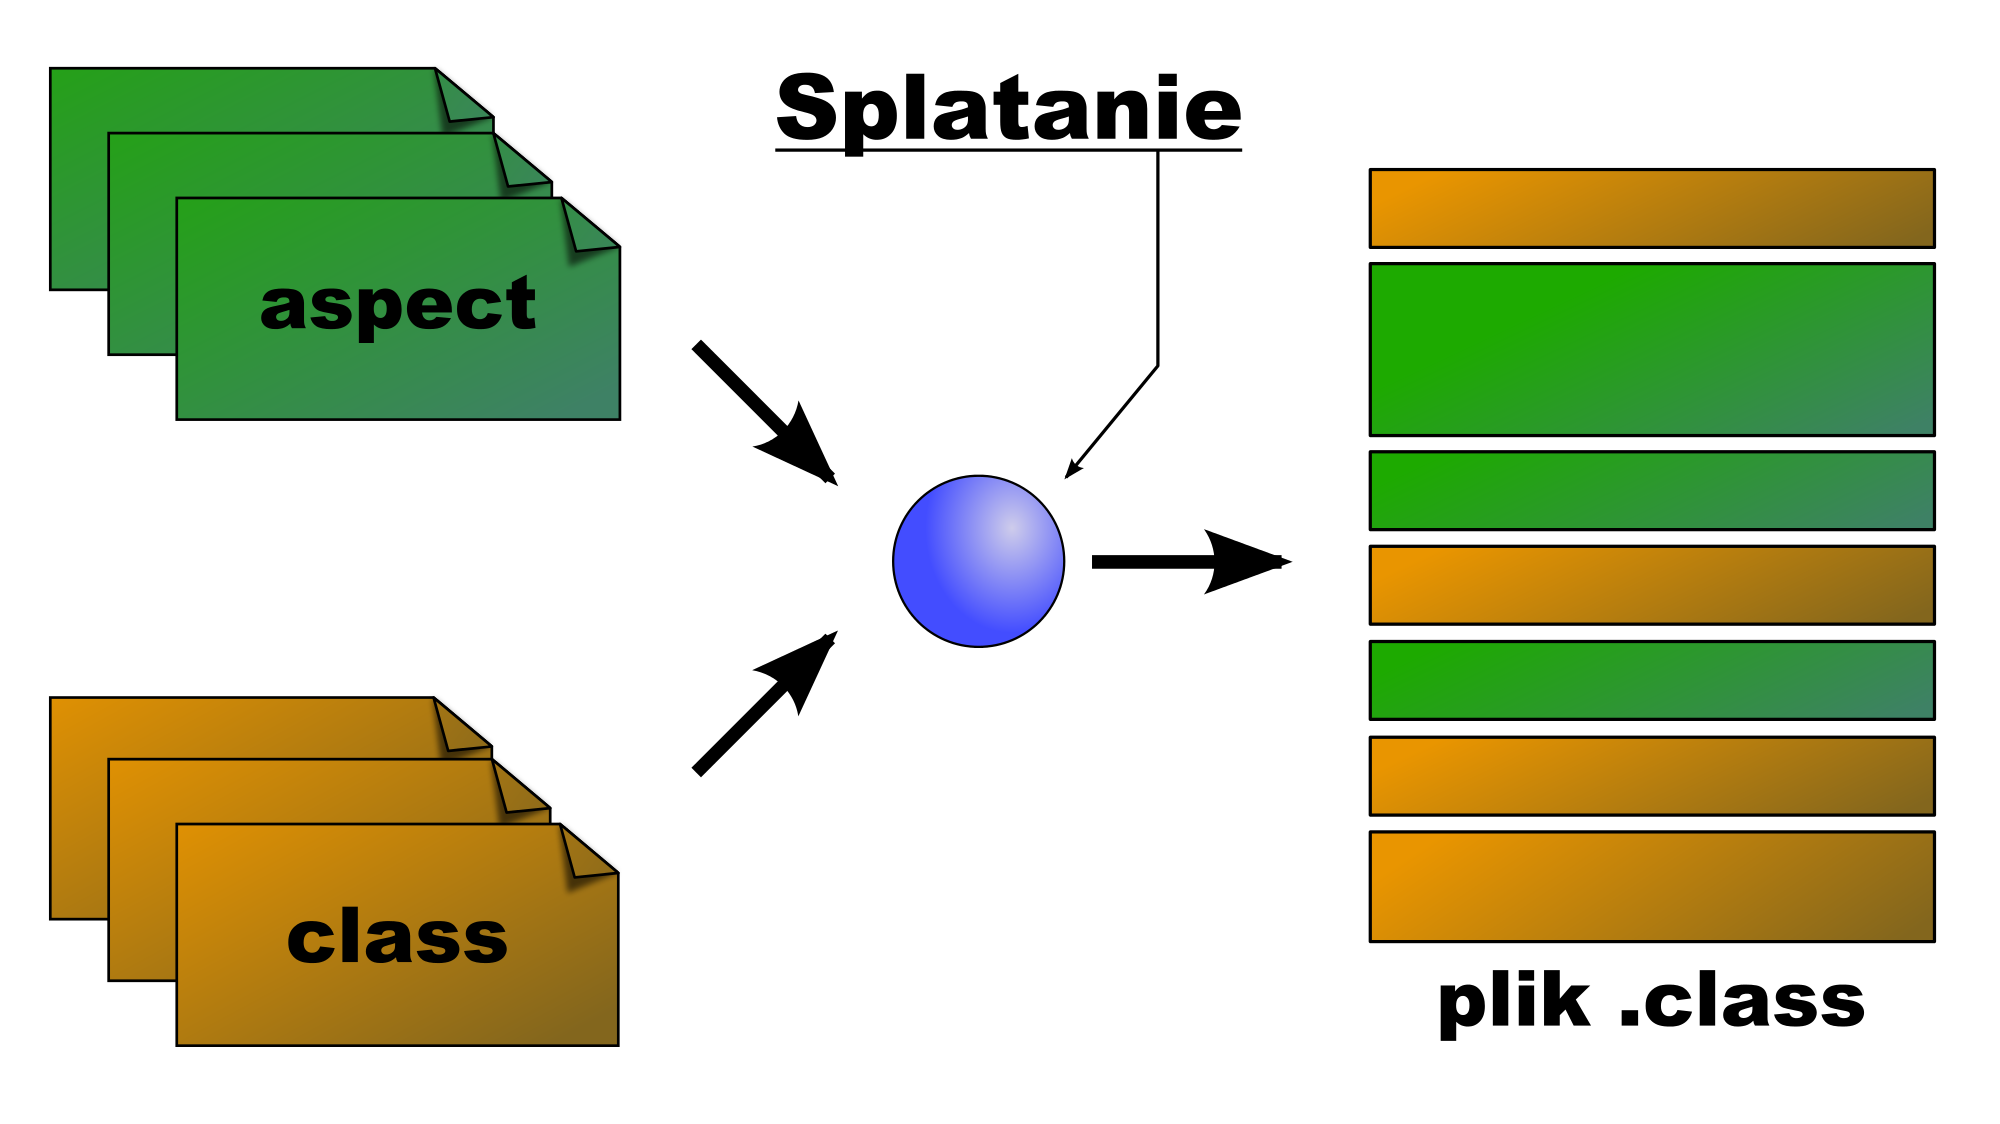
\includegraphics[width=0.80\textwidth]{../images/aspektProgramming.png}
  \caption{Idea stojąca za programowaniem aspektowym}
  \label{fig:aspektProgramming}
\end{figure}

\section{Funkcje zagnieżdżone}
\section{Domknięcia}
\section{Częściowa aplikacja funkcji}
\section{Currying}



\chapter{Zbadanie sposobu realizacji oraz ich siły wyrazu}\label{r:SposobRealizacji}
 








\chapter{Porównanie z innymi językami}\label{r:Porownanie}

W niniejszym rozdziale zostanie przedstawione porównanie jak wygląda szybkość funkcji 
wyższego rzędu w C++11 (z zastosowaniem funkcji anonimowych), w odniesieniu do innych języków.
Do celów porównawczych wybrano język Haskell, który jest językiem funkcyjnym bez efektów ubocznych.
Dokonano również porównania w stosunku do Pythona, który jest językiem interpretowanym i 
ma zaimplementowane wiele funkcji wyższego rzędu w swojej bibliotece standardowej.

W celach porównawczych zostanie wykonane 3 funkcje:
\begin{enumerate}
  \item mapowanie
  \item filtrowanie
  \item agregowanie
\end{enumerate}

Na podstawie tych 3 funkcji (oraz zdefiniowanych przy pomocy lambd funckji przekazanych jako argumenty) postaramy się
zdefiniować jakość wprowadzonych rozwiązań. Jednak określenie jakości wprowadzonych rozwiązań jest ciężkie do zdefiniowania
w formie, która da się dobrze porównać między językami, w pracy zostaną użyte dwie metryki:
\begin{enumerate}
  \item ilość znaków użyta do wygenrowania i wywołania funkcji
  \item szybkość wykonania
\end{enumerate}

\section{Szybkośc wykonania}
Szybkość wykonania poszczególnych programów będzie zbadana przy pomocy progrmu \textit{time}. Używając tego programu otrzymujemy 
3 statystyki: \textit{real}, \textit{user}, \textit{sys}, z których w celach porównawczych użyjemy czsu \textit{user}, który jest 
rzeczywistym czasem spędzonym w trybie użytkownia (\textit{ang. user mode}), a nie trybie jądra (\textit{ang. kernel mode}).

\section{Wydajność funkcji wyższego rzędu w C++11}



Na listingu nr \ref{lst:HigherOrderCPP} możemy zobaczyć przykład implementacji 3 funkcji wyższego rzędu 
z użycie funkcji lambda. 

\begin{listing}[H]
\inputminted[mathescape, linenos, numbersep=5pt, bgcolor=bg, rulecolor=\color{darkgray}, frame=lines, framesep=2mm]{cpp}{../SEM1/fun.cpp}
\caption{Przykład poprawnego i niepoprawnego użycia capture-list w wyrażeniach lambda}
\label{lst:HigherOrderCPP}
\end{listing}



\section{Porównanie z językiem Haskell}
\section{Porównanie z językiem Python}

W tej sekcji zostanie przedstawione te same funkcje wyższego rzędu, tylko że w języku Python. 
Znajdują się one na listingu nr \ref{lst:HigherOrderPython}:
 
\begin{listing}[H]
\inputminted[mathescape, linenos, numbersep=5pt, bgcolor=bg, rulecolor=\color{darkgray}, frame=lines, framesep=2mm]{python}{../SEM1/fun.py}
\caption{Przykład funkcji wyższego rzędu w języku Python}
\label{lst:HigherOrderPython}
\end{listing}









\chapter{Biblioteka LINQ w C++}\label{r:Biblioteka}

Biblioteka LINQ w C++


\chapter{Podsumowanie}



\listoffigures
\listoftables
% \listoflistings

\begin{thebibliography}{99}
\addcontentsline{toc}{chapter}{Bibliografia}

\bibitem[Bea65]{beaman} Juliusz Beaman, \textit{Morbidity of the Jolly
    function}, Mathematica Absurdica, 117 (1965) 338--9.

\bibitem[Blar16]{eb1} Elizjusz Blarbarucki, \textit{O pewnych
    aspektach pewnych aspektów}, Astrolog Polski, Zeszyt 16, Warszawa
  1916.

\bibitem[Fif00]{ffgg} Filigran Fifak, Gizbert Gryzogrzechotalski,
  \textit{O blabalii fetorycznej}, Materiały Konferencji Euroblabal
  2000.

\bibitem[Fif01]{ff-sr} Filigran Fifak, \textit{O fetorach
    $\sigma$-$\rho$}, Acta Fetorica, 2001.

\bibitem[Głomb04]{grglo} Gryzybór Głombaski, \textit{Parazytonikacja
    blabiczna fetorów --- nowa teoria wszystkiego}, Warszawa 1904.

\bibitem[Hopp96]{hopp} Claude Hopper, \textit{On some $\Pi$-hedral
    surfaces in quasi-quasi space}, Omnius University Press, 1996.

\bibitem[Leuk00]{leuk} Lechoslav Leukocyt, \textit{Oval mappings ab ovo},
  Materiały Białostockiej Konferencji Hodowców Drobiu, 2000.

\bibitem[Rozk93]{JR} Josip A.~Rozkosza, \textit{O pewnych własnościach
    pewnych funkcji}, Północnopomorski Dziennik Matematyczny 63491
  (1993).

\bibitem[Spy59]{spyrpt} Mrowclaw Spyrpt, \textit{A matrix is a matrix
    is a matrix}, Mat. Zburp., 91 (1959) 28--35.

\bibitem[Sri64]{srinis} Rajagopalachari Sriniswamiramanathan,
  \textit{Some expansions on the Flausgloten Theorem on locally
    congested lutches}, J. Math.  Soc., North Bombay, 13 (1964) 72--6.

\bibitem[Whi25]{russell} Alfred N. Whitehead, Bertrand Russell,
  \textit{Principia Mathematica}, Cambridge University Press, 1925.

\bibitem[Zen69]{heu} Zenon Zenon, \textit{Użyteczne heurystyki
    w~blabalizie}, Młody Technik, nr~11, 1969.


\end{thebibliography}

\end{document}